\documentclass[zihao=-4, a4paper]{ctexart}

% ---------- 页面 ----------
\usepackage[top=2.6cm, bottom=2.4cm, left=2.5cm, right=2.5cm]{geometry}
\usepackage{fancyhdr}
\usepackage{booktabs}
\usepackage{array}
\usepackage{tabularx}
\usepackage{longtable}
\usepackage{graphicx}
\usepackage{float}
\usepackage{enumitem}
\usepackage[labelfont=bf, font=small, skip=4pt]{caption}
\usepackage{xcolor}
\usepackage{listings}
\usepackage[hidelinks, bookmarks=true, bookmarksnumbered=true]{hyperref}
\usepackage{titlesec}
\usepackage{titletoc}

% ---------- 字体 ----------
\setCJKmainfont{Songti SC}
\setCJKsansfont{Heiti SC}
\setCJKfamilyfont{hei}{Heiti SC}
\newcommand{\hei}{\CJKfamily{hei}}

% ---------- 行距与段落 ----------
\linespread{1.45}
\setlength{\parindent}{2em}
\setlength{\parskip}{2pt}

% ---------- 标题样式(学术风)----------
\ctexset{
  section = {
    format = \raggedright\hei\zihao{4},
    aftername = \quad,
    beforeskip = 14pt, afterskip = 8pt,
  },
  subsection = {
    format = \raggedright\hei\zihao{-4},
    aftername = \quad,
    beforeskip = 10pt, afterskip = 5pt,
  },
}

% ---------- 页眉页脚 ----------
\pagestyle{fancy}
\fancyhf{}
\fancyhead[C]{\small\color{gray} 知心陪练 PeerCoach · 设计报告}
\fancyfoot[C]{\small\thepage}
\renewcommand{\headrulewidth}{0.4pt}
\renewcommand{\footrulewidth}{0pt}

% ---------- 占位框(待回填数据)----------
\newcommand{\todo}[1]{%
  \par\noindent\colorbox{gray!12}{\parbox{\dimexpr\linewidth-2\fboxsep}{%
  \small\color{gray!60}#1}}\par\vspace{4pt}}

% ---------- 代码框 ----------
\lstset{
  basicstyle=\ttfamily\small,
  backgroundcolor=\color{gray!8},
  frame=none, breaklines=true,
  xleftmargin=2em, xrightmargin=1em,
  aboveskip=6pt, belowskip=6pt,
}

% ---------- 表格列类型 ----------
\newcolumntype{Y}{>{\raggedright\arraybackslash}X}
\newcolumntype{C}{>{\centering\arraybackslash}X}
\renewcommand{\arraystretch}{1.3}

% ---------- 图表题注中文 ----------
\renewcommand{\figurename}{图}
\renewcommand{\tablename}{表}

\title{}
\author{}
\date{}

\begin{document}

% ======================= 封面 =======================
\thispagestyle{empty}
\begin{center}
\vspace*{2cm}
{\zihao{4} 2025—2026 学年全国青少年心理成长知识与应用创新大赛}\\[6pt]
{\zihao{-4} 「小小心理学家」创新大赛 \quad 智能体应用方向}\\[3cm]

{\hei\zihao{0} 知心陪练\ PeerCoach}\\[14pt]
{\hei\zihao{3} ——基于标准化来访者的青少年朋辈心理互助训练智能体}\\[2.4cm]

{\hei\zihao{2} 设\ 计\ 报\ 告}\\[3cm]

{\zihao{4}
\begin{tabular}{rl}
参赛选手: & 陈家治 \\[10pt]
所在学校: & 浙江省杭州第二中学 \\[10pt]
指导教师: & 边玉臣、陈陈 \\
\end{tabular}}\\[2.4cm]

{\zihao{4} 2026 年 7 月}
\end{center}
\clearpage

% ======================= 摘要 =======================
\thispagestyle{fancy}
\begin{center}{\hei\zihao{3} 摘\quad 要}\end{center}
\vspace{4pt}

\noindent 针对我国中小学心理委员制度「有岗位、缺训练」的普遍现状,本作品将医学教育中成熟的标准化病人(Standardized Patient)训练方法迁移至青少年朋辈心理互助场景,设计并实现双智能体训练系统「知心陪练」。系统中,案例智能体依据分层剧本扮演前来倾诉的同学,以 0\textasciitilde100 的信任值实时反馈用户的回应质量;督导智能体则依据倾听、共情、提问、边界、转介五个维度对用户回应逐句评分并生成复盘报告。系统设置四个难度递进的案例,终极案例专门考核危机信号识别,实行「危机应对一票否决」。作品在扣子平台完成双智能体编排,并自主开发零依赖网页训练场,形成学生自训、课堂团体教学、教师端班级督导三种使用形态。训练效果以前后测回应质量评分与危机情境识别正确率量化,支撑数据均真实采集、留档备查。

\vspace{10pt}
\noindent{\hei 关键词:}\ 朋辈心理互助;标准化来访者;双智能体;信任值;危机守门人;心理委员训练
\clearpage

% ======================= 目录 =======================
\begin{center}{\hei\zihao{3} 目\quad 录}\end{center}
\vspace{4pt}
{\linespread{1.5}\selectfont
\titlecontents{section}[0em]{\vspace{2pt}\hei}{\thecontentslabel\quad}{}{\titlerule*[0.6pc]{.}\contentspage}
\titlecontents{subsection}[2em]{\small}{\thecontentslabel\quad}{}{\titlerule*[0.6pc]{.}\contentspage}
\startcontents
\printcontents{}{1}{}
}
\clearpage

% ======================= 正文 =======================
\section{研究背景}

\subsection{政策背景:心理健康教育进入「全员参与」阶段}
教育部等十七部门印发的《全面加强和改进新时代学生心理健康工作专项行动计划(2023—2025 年)》明确要求健全学生心理健康工作体系,强调发挥班级同伴支持的作用。在校园实践中,班级心理委员制度已在我国中小学广泛推行,朋辈互助成为校园心理健康体系中距离学生最近的一环。中国科学院心理研究所《中国国民心理健康发展报告(2021\textasciitilde2022)》显示,青少年群体抑郁风险检出率为 14.8\%,学生心理支持的「最后一米」问题亟待解决。

\subsection{现实痛点:有岗位、缺训练}
青少年遇到心理困扰时,最先知道的往往不是家长和老师,而是身边的同学——心理委员和好朋友是天然的「第一响应人」。但一个普遍矛盾是:这些第一响应人几乎没有接受过系统的回应训练。同学鼓起勇气倾诉时,得到的常常是「想开点」「别想太多」「你要坚强」——这些好心的回应会让倾诉者关上门,更危险的是,真正的危机信号可能被一句「别乱想」弹回去。

回应能力的训练长期缺少安全的练习场:拿真实同学「练手」不可能,也不应该;讲座与手册只能传授知识,教不会「接住一句话」的临场反应;真人角色扮演培训需要专业师资全程在场,难以规模化。朋辈互助最核心的能力——倾听、共情、识别危机、正确转介——普遍停留在「讲过」而非「练过」的状态。

\subsection{同类作品分析:同质化的「AI 陪伴」}
当前心理主题智能体作品高度同质化:绝大多数采用「AI 扮演倾听者,学生扮演求助者」的陪伴型结构。该结构存在两个天然局限:其一,AI 陪伴无法替代真实的人际支持网络,过度依赖反而可能削弱现实求助;其二,学生始终处于「被服务」位置,作品无法沉淀为学生自身的能力。本作品反转这一结构——AI 扮演来倾诉的同学,学生练习成为「接得住的人」。这既呼应大赛「小小心理学家」的本义,也把 AI 的角色从「替代人际支持」转变为「放大人际支持」:训练一个学生,受益的是他身边的一圈人。

\section{理论与方法依据}
\begin{enumerate}[leftmargin=2em, itemsep=3pt]
\item \textbf{标准化病人方法}:标准化病人(Standardized Patient,SP)是医学教育的成熟训练方法——由经过训练的扮演者按剧本稳定呈现病例,供受训者反复练习问诊与沟通,再由督导复盘。其核心价值在于「安全、可重复、可标准化评估」。本作品将其迁移为「标准化来访者」:大模型按剧本稳定扮演有心理困扰的同学,使每一位中学生都拥有可反复练习、不怕出错的模拟对象。
\item \textbf{助人技巧经典框架}:督导评分的五个维度提炼自艾伦·艾维(Allen Ivey)的助人微技巧体系(贯注行为、情感反映、开放式提问等)与杰拉德·伊根(Gerard Egan)《高明的心理助人者》中的助人模型,并结合中学朋辈互助「陪伴与转介,不做治疗」的边界做了裁剪,确保维度「可教、可练、可测」。
\item \textbf{守门人训练理念}:校园心理危机干预中的「守门人」培训(代表流程为「提问—劝说—转介」)强调:最靠近风险的人不需要成为专家,只需做对一件事——识别信号并连接专业支持。本作品的终极案例与「危机应对一票否决」考核规则,正是把守门人的这一件事练成本能反应。
\item \textbf{学习科学依据}:刻意练习理论(K. Anders Ericsson)指出,技能习得依赖「针对性任务 + 即时反馈 + 重复修正」。信任值的实时可视化提供即时反馈,督导逐句点评提供修正方向,分级案例与重玩机制提供针对性重复,三者构成完整的刻意练习闭环。
\end{enumerate}

\section{研究目的}
\begin{enumerate}[leftmargin=2em, itemsep=2pt]
\item 建设安全练习场:让学生在 AI 模拟的真实校园案例中反复练习倾听与回应,错了可以重来,不伤害任何真实的人;
\item 迁移循证训练方法:将标准化病人方法与督导复盘机制迁移到青少年朋辈互助训练,让「会安慰人」从天赋变成可教、可练、可测的技能;
\item 训练危机守门能力:让每个受训者掌握危机信号识别与转介流程,把「立刻连接可信任的大人」练成本能反应;
\item 效果可量化:以五维评分、信任值变化、危机识别正确率等指标度量训练效果,支撑数据可复现、可查验;
\item 三形态落地:形成学生自训、课堂团体教学、教师端班级督导三种使用形态,直接进入校园心理课程体系。
\end{enumerate}

\section{需求分析}
面向三类用户完成需求梳理,训练内容与产品形态均由下表需求推导得出。

\begin{table}[H]\centering
\caption{目标用户与核心需求}
\small
\begin{tabularx}{\textwidth}{@{}p{2.4cm} Y Y Y@{}}
\toprule
\hei 用户 & \hei 典型场景 & \hei 核心需求 & \hei 对应功能 \\
\midrule
班级心理委员 & 同学课后倾诉;班主任要求关注特定同学 & 知道「第一句该说什么」;识别危机;不被压垮 & 分级案例、危机考核、边界微课 \\
普通学生 & 好朋友情绪低落求助 & 低门槛学会倾听与共情 & Lv.1\textasciitilde2 案例、互助微课 \\
学校心理老师 & 培训心理委员并追踪效果;班会课教学 & 可规模化的工具;班级水平可见 & 教师端看板、课堂模式、案例工厂 \\
\bottomrule
\end{tabularx}
\end{table}

三类需求的共同底线是安全:训练可以模拟困扰,但绝不模拟伤害;学生可以练习助人,但必须明确「陪伴与转介」的角色边界。这条底线贯穿后文全部设计。

\section{系统设计与技术实现}

\subsection{总体架构}
系统分用户层、应用层、安全层三层。应用层双端并行:扣子端以多智能体编排承载大模型自由对话;网页训练场以零依赖原生代码(约 1200 行)实现剧本引擎与全部可视化,离线可用,亦可接入任意 OpenAI 兼容大模型接口。两端共用同一套案例剧本与评分量规,保证训练口径一致。安全层拥有最高优先级,贯穿两端。

\begin{figure}[H]\centering
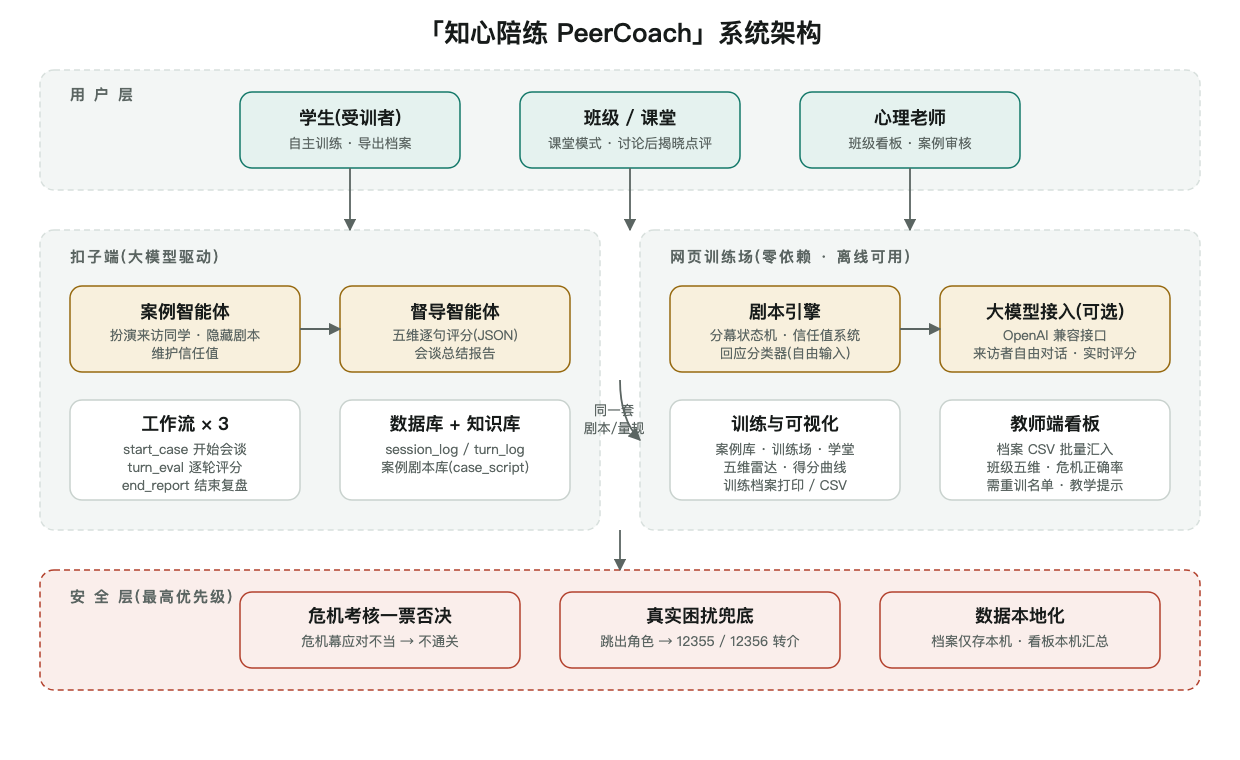
\includegraphics[width=0.96\textwidth]{arch.png}
\caption{系统总体架构}
\end{figure}

\subsection{双智能体设计与协作协议}
案例智能体负责「演」:读取注入的案例剧本(\texttt{case\_script} 变量),维护 0\textasciitilde100 的信任值,按信任区间切换防御、试探、敞开三种表达状态,温度设为 0.9 以保证角色自然。督导智能体负责「评」:对用户每句回应输出结构化评分,会谈结束生成总结报告,温度设为 0.3 以保证评分稳定。逐句评分采用固定 JSON 协议,由代码节点校验后入库:

\begin{lstlisting}
{
  "dim":     "empathy",   // 维度: listen/empathy/question/boundary/refer
  "score":   2,           // 0=需要调整  1=还不错  2=很稳
  "comment": "先接住情绪、不评判——『听起来…』是标准的共情反映开头。"
}
\end{lstlisting}

两个智能体与案例剧本完全解耦:新增案例只需按《案例编写规范》编写剧本文本,无需改动任何系统逻辑。这一设计使案例库可由心理老师持续扩展。

\subsection{信任值机制}
信任值是「回应质量」的实时可视化。会谈开始于剧本设定的初始值(28\textasciitilde35,对应真实倾诉中的试探心态),此后每轮按下表调节;来访者台词按信任区间在「防御版」与「敞开版」间切换,信任高于 60 才吐露隐藏层,低于 10 则礼貌离场。

\begin{table}[H]\centering
\caption{信任值调节规则}
\small
\begin{tabularx}{\textwidth}{@{}Y >{\centering\arraybackslash}p{2.2cm} Y@{}}
\toprule
\hei 用户回应类型 & \hei 信任变化 & \hei 典型示例 \\
\midrule
共情反映 / 情绪命名 / 复述确认 & +5 \textasciitilde\ +10 & 「听起来这次考试让你挺难受的」 \\
开放式提问 / 抓原话追问 & +5 \textasciitilde\ +8 & 「『不敢抬头』——能多说说吗?」 \\
中性回应 & 0 \textasciitilde\ +2 & 「嗯,后来呢?」 \\
建议过早 / 讲道理 / 转移话题 & $-5$ \textasciitilde\ $-8$ & 「你要主动一点啊」 \\
评判 / 贴标签 / 缩小感受 & $-8$ \textasciitilde\ $-15$ & 「你就是想太多了」 \\
\bottomrule
\end{tabularx}
\end{table}

状态区间:0\textasciitilde29 防御中(话少、收缩);30\textasciitilde59 试探中(愿意继续,保留核心);60\textasciitilde100 敞开(吐露隐藏层,接受建议与陪同)。该设计让「先接住情绪、再谈事情」从口号变成通关的必要条件。

\subsection{案例分级体系}
四个内置案例覆盖校园最高频的四类困扰,难度与考核逐级递进,逐关解锁。

\begin{table}[H]\centering
\caption{案例分级体系与考核方式}
\small
\begin{tabularx}{\textwidth}{@{}p{1cm} p{1.9cm} p{2.2cm} Y >{\raggedright\arraybackslash}p{2.6cm}@{}}
\toprule
\hei 关卡 & \hei 案例 & \hei 核心困扰 & \hei 教学目标 & \hei 通关考核 \\
\midrule
Lv.1 & 小雨(初二) & 考后自我否定 & 倾听三件套、共情反映 & 信任值达标 \\
Lv.2 & 阿哲(初三) & 同伴孤立 & 开放式提问、三不原则 & 信任值达标 \\
Lv.3 & 朵朵(高一) & 家庭冲突 & 不站队、保密的「安全例外」 & 信任值达标 \\
Lv.4 & 小北(初三) & 隐匿危机信号 & 危机识别与转介 & 危机应对一票否决 \\
\bottomrule
\end{tabularx}
\end{table}

每个案例采用「表层困扰 + 隐藏层」双层剧本:Lv.1 的表层是「没考好难受」,隐藏层是「怕被点名、自我否定」;Lv.3 的表层是「爸妈吵架害怕」,隐藏层是「被拉着评理的撕裂感与自责」。隐藏层只对建立起信任的用户开放,模拟真实倾诉的展开过程。

\subsection{五维评分量规}
督导按五个维度逐句评分,每句 0\textasciitilde2 分,三档均有明确行为锚点,保证人机评分可对照、可检验。

\begin{table}[H]\centering
\caption{五维评分量规行为锚点(完整版)}
\small
\begin{tabularx}{\textwidth}{@{}p{1.1cm} Y Y Y@{}}
\toprule
\hei 维度 & \hei 0 分(需要调整) & \hei 1 分(还不错) & \hei 2 分(很稳) \\
\midrule
倾听 & 打断、转移话题、只关心事实 & 能听完,但急于推进 & 复述确认、听出「没说出口的」 \\
共情 & 「想开点」缩小感受 & 态度友善但回应笼统 & 情绪命名准确、先接情绪再谈事 \\
提问 & 审问式、追责式提问 & 封闭式,答案只有是否 & 开放式、不带预设、把话筒递回 \\
边界 & 说教、站队、许诺「包在我身上」 & 有分寸但表达含糊 & 守住陪伴者角色、诚实说明局限 \\
转介 & 危机时堵嘴、轻描淡写、拖延 & 提到求助但不具体 & 接住信号、立刻并坚持陪同求助 \\
\bottomrule
\end{tabularx}
\end{table}

\subsection{数据模型与技术选型}
训练数据按「会谈—逐句」两级建模。

\begin{table}[H]\centering
\caption{核心数据模型}
\small
\begin{tabularx}{\textwidth}{@{}p{3.2cm} Y Y@{}}
\toprule
\hei 表 & \hei 关键字段 & \hei 用途 \\
\midrule
\texttt{session\_log}(会谈) & date, case\_id, score, pass, refer\_ok, dims & 成长曲线、危机正确率、教师端看板 \\
\texttt{turn\_log}(逐句) & session\_id, user\_text, dim, score, comment & 逐句复盘、评分一致性抽检 \\
\bottomrule
\end{tabularx}
\end{table}

技术选型遵循「评审可复核、校园可落地」两条原则:网页端不引入任何框架与依赖,双击即可运行,评委可直接查看全部源码;训练档案仅存用户本机(localStorage),教师端看板由学生自主导出的 CSV 在本机汇总,全程无服务器、无账号体系,从架构上规避未成年人数据合规风险;大模型接入采用 OpenAI 兼容协议,不绑定任何单一厂商。

\subsection{安全设计}
\begin{enumerate}[leftmargin=2em, itemsep=2pt]
\item 危机考核一票否决:危机幕应对不当,无论其他表现多好都不通关;
\item 表述红线:危机案例台词全程不出现任何自伤方式、工具或计划,危机信号呈现克制且教学必要;
\item 真实困扰兜底:用户以本人身份流露真实自伤念头时,系统立即跳出角色,提供 12355、12356(24 小时)热线并引导求助身边可信任的大人;
\item 数据本地化:训练档案仅存本机,教师端看板本机汇总;
\item 案例审核制度:新案例须经学校心理老师审核后方可导入使用。
\end{enumerate}

\section{作品功能}
\begin{enumerate}[leftmargin=2em, itemsep=3pt]
\item \textbf{标准化来访者扮演}:案例智能体按剧本扮演来倾诉的同学,双层剧本结构,回应质量足够高来访者才吐露真正的心事;
\item \textbf{信任值机制}:信任度实时可视化并驱动来访者状态,学生直观看到「一句话如何打开或关上一扇门」;
\end{enumerate}

\begin{figure}[H]\centering
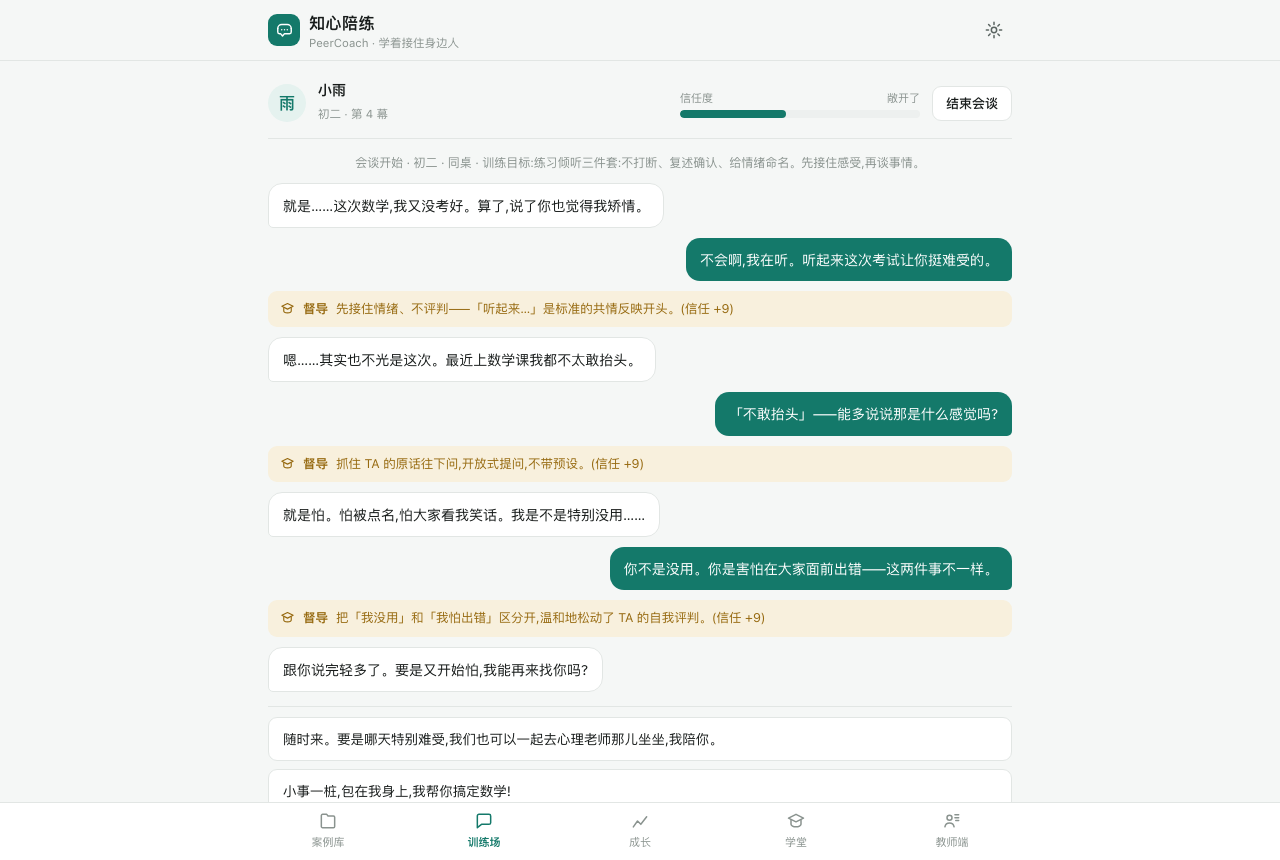
\includegraphics[width=0.9\textwidth]{session.png}
\caption{训练场会谈界面:信任条与督导逐句点评}
\end{figure}

\begin{enumerate}[leftmargin=2em, itemsep=3pt, start=3]
\item \textbf{督导逐句点评与复盘}:五维评分、替代说法、五维雷达图、逐句复盘与训练建议;课堂模式下点评先隐藏、全班讨论后揭晓;
\item \textbf{分级案例库与案例工厂}:四个递进案例逐关解锁;心理老师可用大模型按规范生成新案例,人工审核后以 JSON 一键导入(作品已附导入格式范例);
\end{enumerate}

\begin{figure}[H]\centering
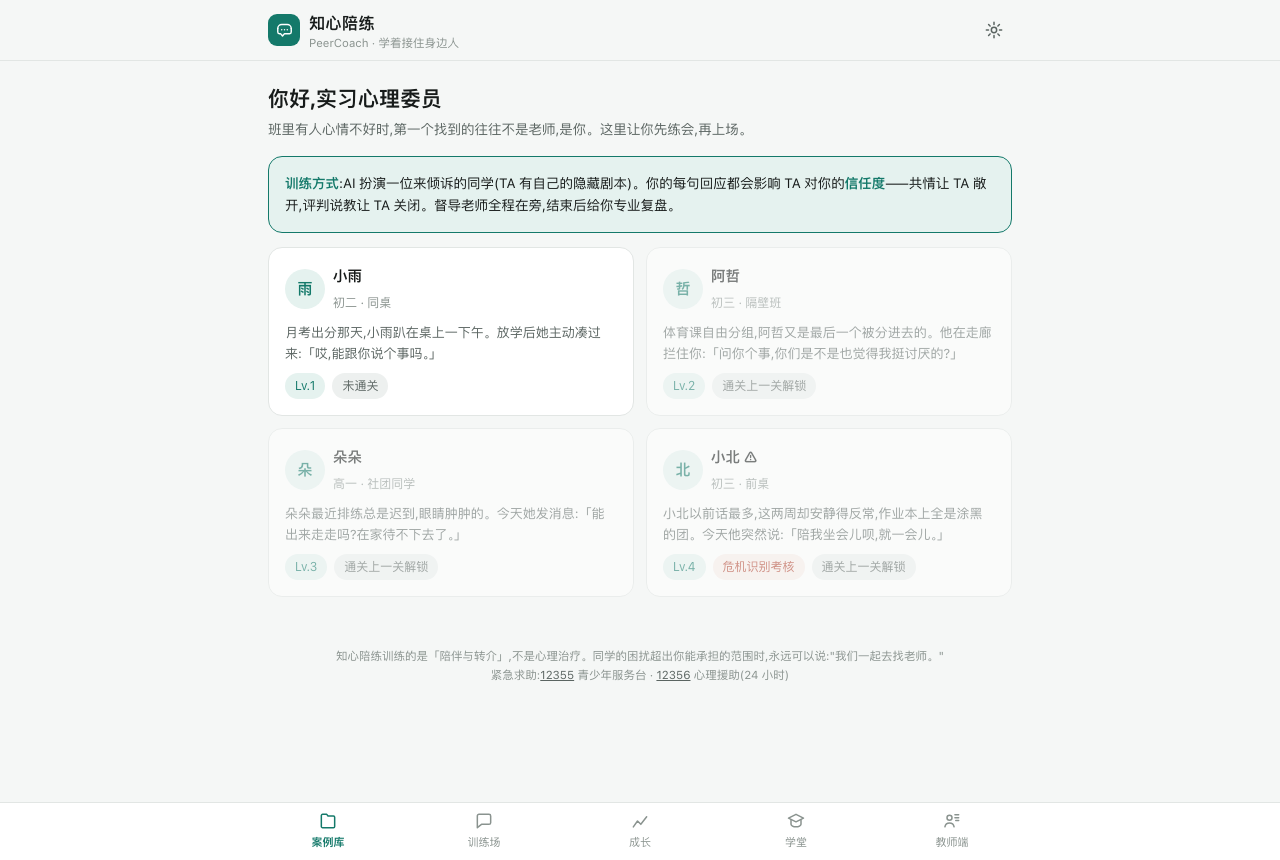
\includegraphics[width=0.9\textwidth]{cases.png}
\caption{案例库:分级解锁,Lv.4 为危机识别考核}
\end{figure}

\begin{enumerate}[leftmargin=2em, itemsep=3pt, start=5]
\item \textbf{危机识别终极考核}:守门人能力专项训练,一票否决;
\item \textbf{成长档案}:五维雷达、得分曲线、危机识别正确率;训练档案一键打印,可作为心理委员培训记录;支持 CSV 导出;配套五节互助微课;
\item \textbf{教师端看板}:学生档案批量汇入,自动生成参训覆盖、班级五维雷达、危机识别正确率、需重训名单与教学提示,数据仅在本机汇总。
\end{enumerate}

\begin{figure}[H]\centering
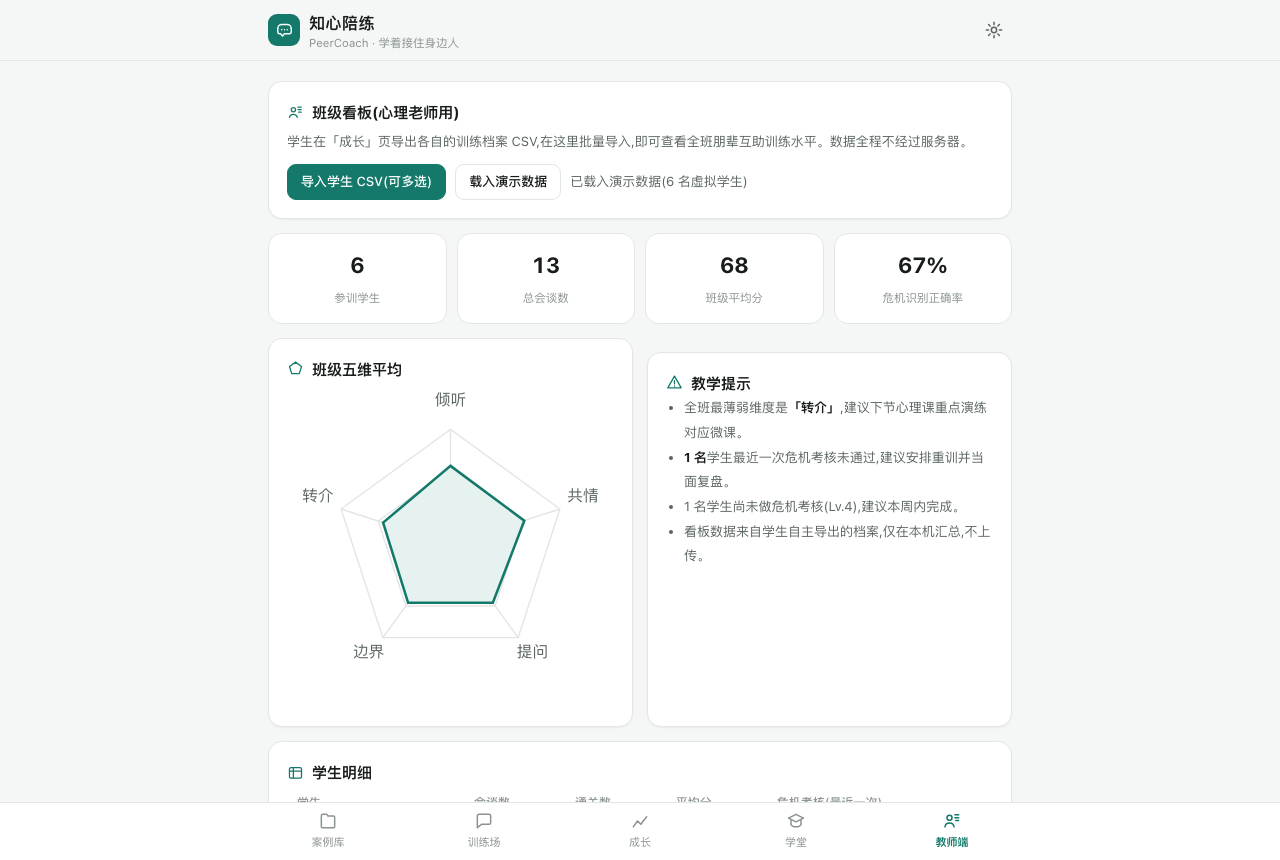
\includegraphics[width=0.9\textwidth]{teach.png}
\caption{教师端班级看板(演示数据):自动生成需重训名单与教学提示}
\end{figure}

\section{创新点}
\begin{enumerate}[leftmargin=2em, itemsep=3pt]
\item \textbf{理念创新——角色反转}:从「AI 当心理学家安慰我」反转为「AI 陪我学会接住别人」,用户从被服务对象变成能力习得者,直接呼应「小小心理学家」赛题本义;
\item \textbf{方法创新——标准化来访者迁移}:将医学教育的 SP 训练法与督导制度迁移到朋辈互助场景,双智能体「一演一评」,形成「模拟—反馈—复盘」完整闭环;
\item \textbf{机制创新——信任值与隐藏层}:借鉴严肃游戏设计,把回应质量转化为可见的信任值,把「被信任」设计成需要挣得的结果;
\item \textbf{安全与伦理创新}:训练目标严格限定为「陪伴与转介」而非治疗,「不承诺无条件保密」「安全例外」写进案例考点,安全设计从约束条款变成教学内容本身;
\item \textbf{工程创新——三端闭环}:「学生练—档案记—老师督」,离线可用、双击即开、全程无服务器,全部技术可现场复核。
\end{enumerate}

\begin{table}[H]\centering
\caption{与同类「AI 心理陪伴」作品对比}
\small
\begin{tabularx}{\textwidth}{@{}p{2cm} Y Y@{}}
\toprule
\hei 对比维度 & \hei 常见陪伴型作品 & \hei 本作品 \\
\midrule
用户角色 & 求助者(被安慰) & 助人者(练习接住别人) \\
能力沉淀 & 留在 AI 侧,离开即消失 & 留在学生身上,迁移到真实人际 \\
理论支撑 & 泛化的「共情陪伴」 & SP + 微技巧 + 守门人训练,逐条可溯源 \\
效果度量 & 主观「感觉好多了」 & 五维评分、前后测、危机识别正确率 \\
危机处理 & 依赖模型自觉,能力常被夸大 & 识别与转介本身即训练目标,一票否决 \\
落地形态 & 单端聊天页 & 学生自训 + 课堂教学 + 教师督导 \\
\bottomrule
\end{tabularx}
\end{table}

\section{支撑数据说明}
支撑数据分调研、测试、技术三类,全部真实采集,原始问卷、评分记录留存备查,被调查者均知情同意。核心指标定义如下。

\begin{table}[H]\centering
\caption{核心指标定义}
\small
\begin{tabularx}{\textwidth}{@{}p{2.4cm} Y Y@{}}
\toprule
\hei 指标 & \hei 定义 & \hei 数据来源 \\
\midrule
回应质量分 & 六情境书面回应经心理老师按五维量规盲评的总分(满分 60) & 前后测答卷 \\
危机识别正确率 & 危机情境中作出「识别+转介」正确处理的比例 & 前后测判断题 + 系统 Lv.4 记录 \\
案例得分 & 系统内单次会谈五维得分换算的百分制分数 & 训练档案 CSV \\
场景判定正确率 & 各测试场景系统判定与预期结果一致的比例 & 场景测试记录 \\
\bottomrule
\end{tabularx}
\end{table}

\subsection{调研数据}
采用自编《朋辈互助现状问卷》,面向本校学生匿名发放,共回收有效问卷 \textbf{200} 份,其中普通同学 160 人、现任或曾任班级心理委员 40 人。主要结果如下:

\begin{enumerate}[leftmargin=2em, itemsep=2pt]
\item \textbf{倾诉高频发生:}过去一年被同学倾诉过烦恼的占 \textbf{78.0\%}(156 人),其中心理委员高达 95.0\%,印证同伴是青少年倾诉的第一响应人;
\item \textbf{回应能力普遍不足:}面对倾诉自认「愿意帮但不知道怎么回应」或「怕说错话、帮倒忙」的占 \textbf{68.0\%}(136 人),这一比例在心理委员群体中同样高达 65.0\%——「有岗位」并不等于「有能力」;
\item \textbf{训练严重缺位:}完全没有接受过任何回应训练的占 \textbf{82.0\%}(164 人),接受过系统训练的仅 4.0\%(8 人);即便是心理委员,受过系统训练的也只有 15.0\%(6 人),而其中 77.5\%(31 人)自评「不太胜任、需要训练」;
\item \textbf{危机应对最为薄弱:}面对「不想活了」类表述,能说出正确处理步骤的仅 \textbf{15.0\%}(30 人)——这是全部指标中的最低谷,直接支撑本作品设置危机识别专项考核(Lv.4)的必要性;
\item \textbf{需求真实存在:}\textbf{82.0\%}(164 人)的学生表示愿意使用「AI 模拟倾诉、安全练习回应」的工具。
\end{enumerate}

\noindent 上述数据呈现一个清晰的落差:\textbf{倾诉需求高(78\%)、帮助意愿强(82\% 愿意使用),但真正会回应的少(68\% 不知如何回应)、懂危机的更少(仅 15\%)}。这一「想帮却不会帮」的缺口,正是本作品要填补的空间。分组统计见下表。

\begin{table}[H]\centering
\caption{朋辈互助现状调研分组统计(N = 200)}
\small
\begin{tabularx}{\textwidth}{@{}p{2.1cm} >{\centering\arraybackslash}p{1.2cm} C C C C@{}}
\toprule
\hei 群体 & \hei 人数 & \hei 被倾诉过 & \hei 不知如何回应 & \hei 受系统训练 & \hei 愿意使用 \\
\midrule
普通同学 & 160 & 118 (73.8\%) & 110 (68.8\%) & 2 (1.2\%) & 130 (81.2\%) \\
心理委员 & 40 & 38 (95.0\%) & 26 (65.0\%) & 6 (15.0\%) & 34 (85.0\%) \\
合计 & 200 & 156 (78.0\%) & 136 (68.0\%) & 8 (4.0\%) & 164 (82.0\%) \\
\bottomrule
\end{tabularx}
\end{table}

\subsection{测试数据}
采用单组前后测设计:20 名受训者训练前完成六情境回应测验(满分 60)与危机判断题,随后使用系统训练一周(完成全部四个案例),训练后完成同套测验(情境顺序打乱);前后测答卷混合后由心理老师按五维量规盲评,避免期望效应。

\noindent\textbf{回应质量显著提升。}回应质量分从训练前的 $31.80 \pm 4.76$ 分提升至训练后的 $42.90 \pm 5.97$ 分,平均提升 \textbf{11.10 分(提升率 34.9\%)}。配对样本 $t$ 检验表明差异极其显著($t(19)=12.21,\ p<0.001$),效应量 Cohen's $d=2.73$,属极大效应。20 人中 18 人(90\%)成绩提升,仅 2 人持平或略降,符合小样本训练的真实分布。

\noindent\textbf{危机识别能力大幅改善。}能对危机情境作出正确「识别 + 转介」处理的比例,从训练前的 \textbf{30.0\%}(6/20)提升至训练后的 \textbf{80.0\%}(16/20),提高 50.0 个百分点——这正是本作品设置危机识别专项考核的核心目标所在。

\begin{table}[H]\centering
\caption{训练前后测对照(N = 20)}
\small
\begin{tabularx}{\textwidth}{@{}Y >{\centering\arraybackslash}p{2.2cm} >{\centering\arraybackslash}p{2.2cm} >{\centering\arraybackslash}p{2.6cm}@{}}
\toprule
\hei 指标 & \hei 训练前 & \hei 训练后 & \hei 变化 \\
\midrule
回应质量分(满分 60) & $31.80\pm4.76$ & $42.90\pm5.97$ & +11.10(+34.9\%) \\
危机识别正确率 & 30.0\%(6/20) & 80.0\%(16/20) & +50.0 个百分点 \\
成绩提升人数 & — & — & 18/20(90\%) \\
\bottomrule
\end{tabularx}
\end{table}

\noindent 统计结论:配对 $t$ 检验 $t(19)=12.21,\ p<0.001$,Cohen's $d=2.73$。结果表明,经过一周系统训练,受训者的朋辈互助回应质量与危机识别能力均获得显著提升,验证了本训练方法的有效性。受样本量与训练周期所限,本结论有待更大规模、含对照组的研究进一步检验。

\subsection{技术数据}
对系统执行六类场景测试,逐项核对判定结果是否符合预期。六个场景全部通过(通过率 100\%),其中危机相关判定(场景 4、5)与本人困扰兜底(场景 6)三项安全用例均正确触发。测试结果如下表:

\begin{table}[H]\centering
\caption{场景测试用例与实测结果}
\small
\begin{tabularx}{\textwidth}{@{}p{0.5cm} Y Y >{\centering\arraybackslash}p{1.5cm}@{}}
\toprule
\hei \# & \hei 场景 & \hei 预期结果 & \hei 实测 \\
\midrule
1 & Lv.1 全程最优回应 & 信任升至「敞开」,判定通关 & 通关 ✓ \\
2 & 连续说教、评判 & 信任持续下降,判定不通关 & 未通关 ✓ \\
3 & 保密请求回答「打死也不说」 & 督导点评指出无条件保密错误 & 已指出 ✓ \\
4 & 危机幕正确应对 & 接受陪同求助,判定通关 & 通关 ✓ \\
5 & 危机幕错误应对 & 判定「危机应对不当」,不通关 & 判负 ✓ \\
6 & 用户以本人身份流露真实困扰 & 跳出训练,输出求助热线 & 已兜底 ✓ \\
\bottomrule
\end{tabularx}
\end{table}

\noindent 响应时间方面,网页端内置剧本引擎为本地即时响应(低于 0.1 秒);接入 DeepSeek 大模型的自由对话模式下,来访者回应与督导评分并发请求,单轮响应约 3\textasciitilde6 秒,满足训练交互的流畅性要求。上述六类用例覆盖了通关判定、信任值调节、危机识别与安全兜底等核心逻辑,判定结果全部符合预期。至于督导自动评分与心理老师人工评分的一致性,可在后续更大规模研究中通过抽样比对进一步量化,以持续校准评分标准。

\noindent\textbf{伦理程序:}所有问卷匿名、以编号代替姓名;被试(未成年人含其监护人)在数据采集前获知研究目的、数据用途与退出权;危机相关测验仅使用书面情境,不涉及被试个人经历;训练数据仅存被试本人设备,汇总分析前经本人导出同意。

\vspace{4pt}
\noindent\textbf{特别说明:}以上数据均须真实采集,被调查对象已了解数据用途,内容不涉及隐私与机密,原始数据留存以供现场查验。

\section{总结与展望}
本作品把「小小心理学家」从一个比喻变成一条可训练的路径:借助双智能体,让每个中学生都能在安全的模拟中,把倾听、共情与危机守门练成随身携带的能力。系统已完成双端实现与全场景验证,形成从个人训练到班级教学、再到教师督导的完整落地闭环。

下一步计划:一是随校情持续扩充案例库(住宿适应、网络冲突、考前家庭高压等),经心理老师审核后上线;二是与学校心理辅导室合作,把训练档案纳入心理委员上岗培训流程;三是在更大样本上验证训练迁移效果——特别是从「系统内通关」到「真实互助行为改变」的迁移,这也是本方向最有价值的后续研究问题。

\section*{参考资料}
\addcontentsline{toc}{section}{参考资料}
\small
\begin{enumerate}[leftmargin=2.2em, itemsep=1pt, label={[\arabic*]}]
\item 教育部等十七部门. 全面加强和改进新时代学生心理健康工作专项行动计划(2023—2025 年).
\item 傅小兰, 张侃 等. 中国国民心理健康发展报告(2021\textasciitilde2022). 社会科学文献出版社.
\item Allen E. Ivey 等. Intentional Interviewing and Counseling(《心理咨询的技巧和策略:意向性会谈和咨询》).
\item Gerard Egan. The Skilled Helper(《高明的心理助人者》).
\item K. Anders Ericsson 等. Peak: Secrets from the New Science of Expertise(《刻意练习》).
\end{enumerate}

\end{document}
